\section{Overview}
\label{sec:overview}

\subsection{Threat Model}

% Move to introduction.tex in order to place it on the 2nd page.
\begin{figure*} 
\begin{center} 
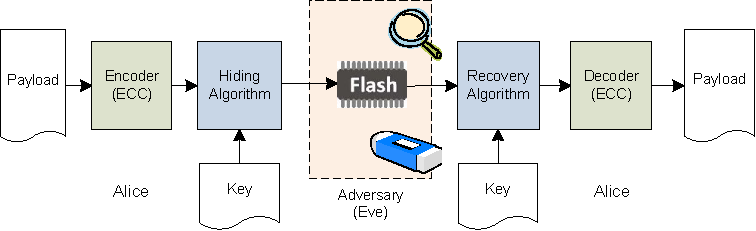
\includegraphics[width=6.5in]{figs/overview.pdf} 
%\includegraphics[width=3.0in]{figs/eval_performance_diff_context.pdf} 
\caption{The overview of the information hiding operation.}
\label{fig:overview} 
\end{center} 
\end{figure*} 

Figure~\ref{fig:overview} shows the overview of the information hiding
process in Flash memory. In order to hide information in Flash, Alice (left)
first adds an error correcting code (ECC) to her message payload and hides the
payload in the analog characteristics in Flash memory. Later, Alice (right) can
perform the reverse operations to retrieve the hidden payload by recovering
bits from the analog characteristics and correct errors using the ECC.
The information hiding and recovery algorithms use a secret key (hiding key)
%, often called {\em stego-key}, 
to determine where the hidden bits are stored in Flash memory. 
As error correcting codes are well studied, this paper focuses on the
physical encoding and decoding of information in Flash.

%As shown in the figure, the information hiding
%can be seen as a communication between two parties, from Bob (left) to
%Alice (right) in the figure \cite{simmons83}. 

As shown in the figure, an adversary (Eve) gets temporary access
to the Flash memory after Alice hides information. We assume that the adversary can inspect
and manipulate the memory through its normal interface, but do not consider physical
tampering of the memory. In the simple case, the adversary can check normal Flash operations
such as program, erase, and read operations. The adversary may also be aware of the information
hiding technique and can specifically check analog characteristics of Flash memory that
can be observed through the standard interface. 

The goal of the adversary may differ depending on the target application. In particular, the
adversary may try to
\begin{itemize}
\item Detect the existence of hidden information,
\item Retrieve the hidden information, or
\item Remove the hidden information.
\end{itemize}
For example, in the traditional steganography context where Alice is trying to establish 
a covert communication channel, it is important that the adversary cannot easily detect
the existence of hidden information. On the other hand, in the context of storing sensitive
information, it is more important that the adversary cannot retrieve information without
knowing the hiding key. For watermarking, it should be difficult to erase the hidden information.

Given an unlimited amount of time with the Flash chip, an adversary can break the information
hiding scheme by trying the retrieval algorithm on all pages with all possible hiding key values
because we assume that an adversary knows our hiding algorithm.
Therefore, the goal of the hiding technique is to make the detection, retrieval, and removal
of hidden information sufficiently time consuming for an attacker. 



%The proposed information hiding technique aims to enable reliable and
%secure communications. First, Bob should be able to reliably
%recover the hidden payload (in other words, the bit error rate after
%the recovery algorithm should be low enough to be corrected by the ECC).
%Second, it should be difficult for Eve to check whether there is
%hidden information or not, or recover the hidden information without
%the stego-key.
%Third, it should be difficult to for Eve to remove the hidden information.

%In this paper, we consider two types of adversaries. In the first case,
%an adversary is not aware of the proposed information hiding technique
%and only checks normal Flash operations and content. In this scenario,
%information hiding is successful if the hidden information cannot be found
%or removed by inspecting or erasing the Flash content. The proposed
%technique easily meets these conditions because hidden information is
%not encoded in the data stored in Flash memory.


%Interface - what is assumed about the interface. Abort function.
\subsection{Flash Interface Requirements}

The proposed technique is designed to work with Flash or other floating-gate 
non-volatile memory, as long as one can control read, program (write), and erase 
operations to specific memory locations (pages and blocks), issue the RESET 
command, and disable internal ECC (if there is any). 
For example, our experiments use off-the-shelf Flash chips that
use the Open NAND Flash Interface (ONFI) \cite{onfi}, which is used by 
many major Flash vendors including Intel, Hynix, Micron, and SanDisk. Other 
Flash vendors such as Samsung and Toshiba also use similar interfaces to their chips. 
In many embedded and mobile devices, the required interface functions are already
exposed to the software layers so that the proposed technique can be simply implemented
as a software update.

%Embedded systems typically implement a Flash memory controller in software, exposing the low-level Flash chip interface to a software layer. Our prototype USB board in the evaluation section is an example of such a design. While we did not have a chance to study details, the manual for the TI OMAP processor family \cite{instruments2013omap}, which is widely used in mobile phones, indicates that its External Memory Interface (EMI) requires software to control each phase of NAND Flash accesses. In such platforms where Flash accesses are controlled by software, our techniques can be implemented as relatively simple software changes. 

